%% LyX 2.0.6 created this file.  For more info, see http://www.lyx.org/.
%% Do not edit unless you really know what you are doing.
\documentclass[english]{article}
\usepackage[T1]{fontenc}
\usepackage[latin9]{inputenc}
\usepackage{float}
\usepackage{graphicx}

\makeatletter

%%%%%%%%%%%%%%%%%%%%%%%%%%%%%% LyX specific LaTeX commands.
%% A simple dot to overcome graphicx limitations
\newcommand{\lyxdot}{.}


\makeatother

\usepackage{babel}
\begin{document}

\title{Exact computation for Ising model for 1D and 2D}

\maketitle
This is short theoretical explanation of the test: \textbf{IsingTestExact1D.h}
and \textbf{IsingTestExact2D.h}.


\section{Combinatorial approach}

We calculate exact solution of specific heat by finding the exact
value of the partition function 
\begin{eqnarray*}
Z(\beta) & = & \sum_{\{\mathrm{all\, configurations\,\sigma_{i}}\}}e^{-\beta E\left(\sigma_{1},\sigma_{2},...,\sigma_{n}\right)}.
\end{eqnarray*}


To do that we have to evaluate all possible configurations of spins.
For given number $n$ of spins on the lattice we have $2^{n}$ configurations.
For example for two spins chain we have
\begin{eqnarray*}
\mbox{} & \left\{ \uparrow\uparrow,\downarrow\uparrow,\uparrow\downarrow,\downarrow\downarrow\right\}  & .
\end{eqnarray*}


Note that some of those configurations may have the same energy $E$,
thus $Z$ function can be written in a bit different way
\begin{equation}
Z(\beta)=\sum_{E_{i}}N(E_{i})e^{-\beta E_{i}},\label{eq:z}
\end{equation}


where the sum runs over all possible energies $E_{i}$, and $N(E_{i})$
is density of states: number of states with the same energy $E_{i}$. 

To generate $N(E)$ we have to calculate $E$ for all configurations
of spins. In order to do that we use Gray code enumeration of spins
(the description of the algorithm can be found e.g. in textbook: \emph{Statistical
Mechanics Algorithms and Computations}, Werner Krauth). The pseudo-code
of the algorithm is following: 

\begin{figure}[H]


\begin{centering}
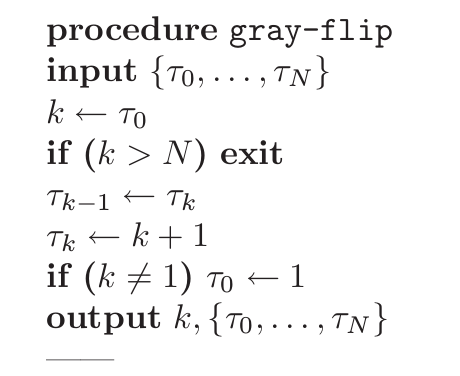
\includegraphics[width=0.2\paperwidth]{GrayCode}
\par\end{centering}

\caption{Gray code for spins $\{0,....,N-1\}$ (which means that the first
spin has index 0). The procedure returns $k$ which is the index of
next spin to flip. $\tau$ is an auxiliary vector used by the procedure.
The initial value of $\tau_{i}=i$ , where $i=(0,1,....,N)$. Look
in the code of IsingTestExact class to see how to use it in practice.
Many execution of the method will create following sequence of spins
to change: (0,1,0,2,0,1,0,3,0,1,0,2,0,1,0,4,....)}


\end{figure}


 We will use binary representation of spin on lattice (i.e. 0 - negative
spin and 1 positive spin). The algorithm will flip one spin (bit),
thus we can calculate the change of energy and the use again gray-flip
method to flip to another configuration. %
\footnote{The algorithm that perform such enumerations are called Gray codes
- in which each configuration differs from its predecessor by one
spin only.%
} For example let us consider three spins system ($\sigma_{0},\,\sigma_{1},\,\sigma_{2}$):
\begin{enumerate}
\item We initialize the $\tau$ array with values: $\tau=(0,1,2,3)$, and
set the initial configuration of spins to $(-1,-1,-1)$ which in binary
representation is $(0,0,0)$.
\item Below we present the table of spins which we have to flip after each
execution of the gray-flip method:
\begin{eqnarray*}
\mathrm{number\, of\, execution} & \mathrm{spin\, to\, change} & \mathrm{configuration}\\
1 & 1 & (1,0,0)\\
2 & 2 & (1,1,0)\\
3 & 1 & (0,1,0)\\
4 & 3 & (0,1,1)\\
5 & 1 & (1,1,1)\\
6 & 2 & (1,0,1)\\
7 & 1 & (0,0,1)
\end{eqnarray*}

\item For each configuration we have to calculate energy $E$ and $N(E)$.
\end{enumerate}
Having the $N(E)$ allows us to calculate all properties of the system
from (\ref{eq:z}). As an example we calculated plots of specific
heat $C_{V}$ in function of temperature $T$. The specific heat is
given by expression 
\[
C_{V}=\frac{\partial\left\langle E\right\rangle }{\partial T},
\]


where $\left\langle E\right\rangle =-\frac{\partial\log(Z)}{\partial\beta}=T^{2}\frac{\partial\log(Z)}{\partial T}$.
Thus we have
\[
C_{V}=2T\frac{\partial\log(Z)}{\partial T}+T^{2}\frac{\partial^{2}\log(Z)}{\partial T^{2}}.
\]


For simplicity we calculate $C_{V}$ using numerical differentiation
using the finite difference method, which leads to following approximation
\begin{eqnarray*}
C_{V} & \left(T\right)\approx & 2T\left(\frac{\log\left(Z(T+\Delta T)\right)-\log\left(Z(T-\Delta T)\right)}{2\Delta T}\right)\\
 & + & T^{2}\left(\frac{\log\left(Z(T+\Delta T)\right)+\log\left(Z(T-\Delta T)\right)-2\log\left(Z(T)\right)}{\Delta T^{2}}\right).
\end{eqnarray*}


We choose small value of $\Delta T=0.01$ (here we consider only small
lattices, this guarantee that the value of $\Delta T$ is small enough
to provide good approximation of derivatives even near the critical
point) which should give us accurate approximation of $C_{V}$. 

Note that this approach gives us exact solution to 2D Ising model,
but it is limited to very small lattice sizes. The bottleneck of the
algorithm is the part where we calculate $N(E)$ using Gray code.
This is because we have to run over $2^{n}$ states which for lattice
of size $6\times6$ gives $2^{36}=68\,719\,476\,736$ number of possible
configurations. 


\section{Results for 1D chain}

The appropriate test class has name: \textbf{IsingTestExact1D}.

We calculate specific heat for three different chain lengths: N=\textbf{2,
7} and \textbf{22}. We also compared this with analytical one. For
1D the partition function is given by following equation
\[
Z\left(T\right)=\left(2\cosh(\beta J)\right)^{N}\cdot\left(1+\tanh(\beta J)^{N}\right),
\]


from this we can calculate $C_{V}$ per spin
\begin{equation}
C_{V}^{\mathrm{spin}}(T)=\frac{T}{N}\frac{\partial^{2}T\log\left(Z\left(T\right)\right)}{\partial T^{2}}.\label{eq:analitycal}
\end{equation}


The numerical approximation of derivative above can be found in function
\textbf{exacCv()}.

The results for exact solution (Combinatorial approach) and analytical
solution (\ref{eq:analitycal}) are shown in the picture below. From
this we see that both methods lead to the same values which is not
a surprise. 

\begin{figure}[H]
\begin{centering}
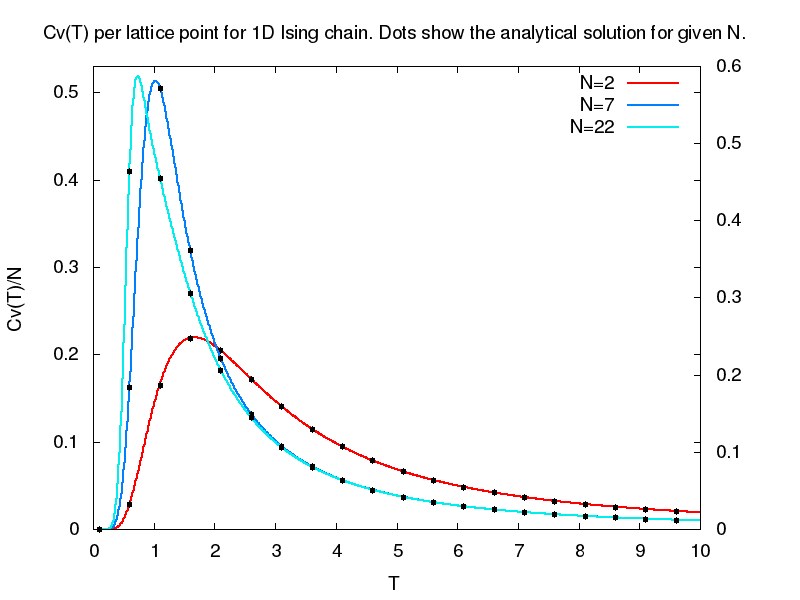
\includegraphics[width=0.4\paperwidth]{\lyxdot \lyxdot /\lyxdot \lyxdot /tests_out/IsingTestExact1D}
\par\end{centering}

\caption{Specific heat for 1D Ising chain for N=2, 7 and 22. The plot is generated
by IsingTestExact1D class.}


\end{figure}


From the picture above we see that for large temperatures ($T\rightarrow+\infty$)
$C_{V}$ tends to zero. We have the same behavior for $T\rightarrow0$. 


\section{Results for 2D chain}

The appropriate test class has name: \textbf{IsingTestExact2D}.

The analytical solution for 2D lattice exist but is more complicated
thus we plot only the results from the combinatorial method. This
method allowed us to calculate lattices up to 5x5. The results are
presented below. In this case we compare our exact calculation with
MC data obtained from our program.

\begin{figure}[H]
\begin{centering}
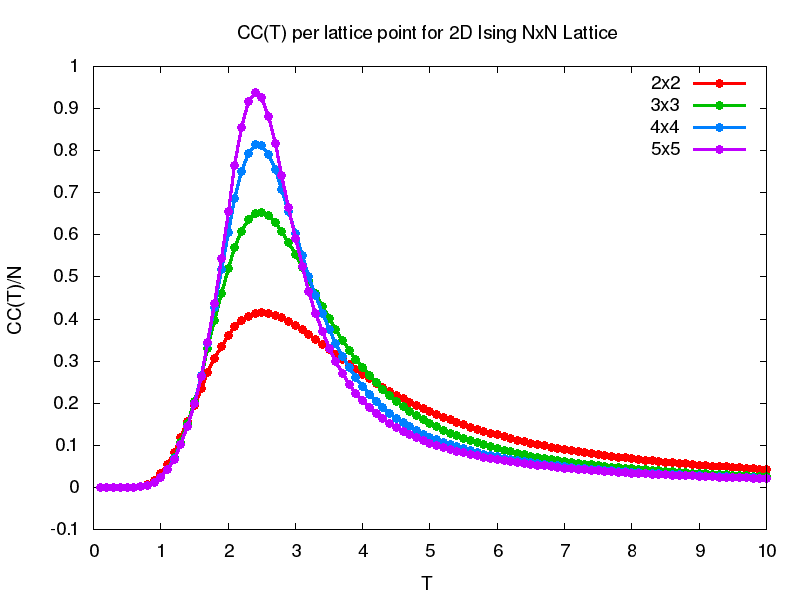
\includegraphics[width=0.4\paperwidth]{\lyxdot \lyxdot /\lyxdot \lyxdot /tests_out/IsingTestExact2D}
\par\end{centering}

\caption{Specific heat for 2D Ising lattice for four different lattices size.
The black dots show the results obtained from MC simulation by Wolff
algorithm (for 5000 MC cycles). The plot is generated by IsingTestExact2D
class. Vertical line shows the exact value of critical temperature
$T_{C}$. }
\end{figure}


From figure above we see that the phase transition for small lattices
occurs near the critical temperature $T_{C}$ obtained from exact
Onsager calculations. For 2D lattice we have the same asymptotic behavior
($T\rightarrow0$ and $T\rightarrow+\infty$) like it was in case
of 1D chain. 

The numerical values of $C_{V}$ from picture above can be reproduced
by test: \textbf{IsingTestCC2D.h}.
\end{document}
